% Compile with pdfLaTeX twice. No date appears in the title block.
\documentclass[conference,a4paper]{IEEEtran}
\usepackage[T1]{fontenc}
\usepackage[utf8]{inputenc}
\usepackage{amsmath,graphicx,booktabs,cite}
\usepackage[hidelinks]{hyperref}
\hypersetup{pdftitle={Sparse4D Battery CT Reconstruction},pdfauthor={Amikula Pavan Kumar Goud}}
\title{Sparse4D Battery CT Reconstruction\\Simulation Validation and Measured Projection Replay}
\author{\IEEEauthorblockN{Amikula Pavan Kumar Goud}
\IEEEauthorblockA{MSc Computer Science Student\\Blekinge Institute of Technology\\Karlskrona, Sweden}}
\begin{document}
\maketitle


\begin{abstract}

This report investigates sparse-view battery computed tomography through simulated NMC electrode experiments and archived Waygate measurements. A compact residual 3D U-Net is trained on 24 spatial regions, selected using six validation regions, and tested on six further regions from one scan. The model with three SIRT steps reduces mean voxel RMSE by 37.64\% against SIRT23; a frozen 2000bar-stack check gives 35.38\%. Gains decline with additive Gaussian noise. Transfer of the NMC model to measured Waygate views instead increases fit projection RMSE by 5.11\%. Physics-only diagnostics at 256 cubed compare 75 to 1200 views: the 300-view reconstruction takes 0.271 s, while 1200 views take 0.534 s in recorded individual runs. Interactive tools expose images, metrics, and assumptions. The evidence establishes a research prototype for fast archived reconstruction, not calibrated live acquisition, defect detection, or specimen-independent generalization.

\end{abstract}

\begin{IEEEkeywords}

Sparse-view computed tomography, cone-beam reconstruction, battery imaging, FDK, SIRT, residual 3D U-Net, GPU acceleration, simulated projections, domain shift, data consistency, reproducibility, interactive visualization.

\end{IEEEkeywords}

\section{Introduction}

Battery CT reconstructs internal structure from X-ray measurements taken at multiple angles. The practical question in this project is whether sparse-view reconstruction can preserve useful detail while remaining fast enough for an interactive engineering workflow. The study combines simulated electrode data with archived measurements from a cylindrical battery, and separates image fidelity from solver latency.

Sparse4D is the project name; the experiments documented here estimate static 3D volumes. Temporal 4D reconstruction, defect classification, state-of-health prediction, and live scanner integration are not demonstrated. This distinction prevents the project title from implying an evaluated capability.

The contributions are a reproducible NMC training pilot with fixed spatial splits; a frozen transfer and Gaussian sensitivity study; a measured-data replay with explicit provisional geometry; a controlled FDK study of view count and voxel resolution; and interfaces that expose images, metrics, provenance, and limitations \cite{ref10}. Negative transfer results are retained alongside improvements.

\section{Background And Related Work}

FDK provides an approximate filtered-backprojection reconstruction for circular cone-beam acquisition \cite{ref1}. The project uses the GPU implementation in ASTRA, whose projection and backprojection primitives support algorithm development \cite{ref2}, \cite{ref3}. SIRT repeatedly reduces projection residuals, with a non-negativity constraint in the iterative experiments. The subsequent view-count diagnostics use FDK alone; their runtimes are not SIRT or hybrid runtimes.

The learned component adapts encoder-decoder and skip-connection ideas from volumetric U-Net \cite{ref4} to regression, and predicts a correction added to an initial reconstruction. Residual learning is a broader architectural principle \cite{ref5}. Direct inversion followed by learned artifact correction is established in imaging literature \cite{ref6}. Those publications motivate design choices; their reported performance is not evidence of performance on this project.

The implementation uses PyTorch for learned correction \cite{ref7} and ASTRA for physics operations. The NMC grayscale stack is obtained from the Battery 3D Images collection \cite{ref8}. The Waygate dataset contains acquired projections and a vendor reconstruction, enabling a distinct measured-data investigation \cite{ref9}.

\section{Data And Evaluation Design}

\subsection{NMC electrode volumes}

Each NMC stack has 218 unique single-page TIFF slices of shape 2048 by 2048 and dtype uint16. Duplicate ZIP entries were identified before extraction; 436 archive entries were not counted as 436 independent slices. The 0bar stack supplies training, validation, and test regions; the 2000bar stack supplies a frozen separate-stack check and the noise sensitivity check.

The fixed 0bar split contains 24 training, 6 validation, and 6 test regions of 128 cubed. All use z indices [45,173), six y origins from 256 to 1216 in steps of 192, and split-specific x strips. Training x origins are 256, 448, 640, and 832; validation and test x origins are 1408 and 1728. Regions are non-overlapping, but all belong to one scan. A previously evaluated central region was excluded. This reduces direct spatial leakage without establishing specimen independence.

Synthetic line integrals are generated with 75 noiseless views, angles 0 to 355.2 degrees in 4.8-degree steps, and a 250 by 250 detector. TIFF intensities are mapped by uint16/65535 times 0.4. The assumed crop width is 12.000041 mm, so 128 voxels correspond to 0.0937503 mm. These values define the simulator; they do not establish physical calibration of the NMC data.

\subsection{Measured Waygate archive}

The 750-pixel Waygate archive contains 1201 projection TIFFs; acquisition and reconstruction metadata specify 1200 usable views. Images 1 through 1200 span 0 to 359.7 degrees at 0.3-degree spacing; image 1201 at the repeated endpoint is excluded. The log timestamps show a first-to-last-used span of 1199 s. Sparse subsets cover the same completed acquisition, rather than demonstrating faster capture.

The vendor reference has 750 cubed voxels and a reported voxel size of approximately 0.03200011 mm. A supplied middle TIFF is a processed 750 by 750 uint16 reconstruction. It is used for context, not as independent physical truth or as a calibrated voxel scoring target \cite{ref9}, \cite{ref10}.

\section{Reconstruction And Training Methods}

\subsection{Physics and learned correction}

For a reference volume x and forward operator A, the simulation is $y = Ax$; noisy sensitivity tests use $y = Ax + e$. The baseline first runs FDK, then 20 SIRT iterations with MinConstraint = 0. Its output undergoes a float16 round trip and is restored to float32 to reproduce the model input. The raw prediction is $x_{\mathrm{raw}}=x_{20}+f_{\theta}(x_{20})$. The hybrid adds three SIRT iterations to this prediction. The matched physics control also adds three iterations, yielding SIRT23.

The correction network uses one input/output channel, encoder widths 12, 24, and 36, two 3 by 3 by 3 convolutions with GELU per block, stride-2 downsampling, trilinear upsampling, and concatenated skip features. A 1 by 1 by 1 output head starts at zero, making initialization an identity correction. It is a compact residual U-Net adaptation, not a reproduction of the segmentation architecture in \cite{ref4}.

Inference uses 80-cubed patches with origins [0,40,48] on each axis, for 27 tiles per 128-cubed region. A separable Hann weight, floored at 0.05 on each one-dimensional window, blends overlaps. Inputs are divided by 0.4 before prediction and outputs rescaled by 0.4. Tiling limits working memory and avoids hard seams.

\subsection{Optimization and checkpoint locking}

Training uses AdamW with learning rate 0.0002 and weight decay 0.0001, 12 epochs, two random 80-cubed patches per update, and six updates per training region per epoch. Right-angle rotations in the XY plane and random Z flips augment paired input/target crops. Mixed precision and gradient clipping at norm 1 are applied. The fixed seed is 20261004.

The normalized loss is L = mean absolute voxel error + 0.1 times the mean absolute discrepancy of first differences along the three spatial axes. Fixed validation patches select the checkpoint; epoch 0 is eligible. Test regions are evaluated only after locking. The selected checkpoint is epoch 12. Validation loss decreases from 0.006895 to 0.005726. These loss values are not voxel RMSE.

\subsection{Gaussian sensitivity experiment}

The frozen epoch-12 model is evaluated on six fresh 2000bar regions at noise fractions 0, 0.01, 0.03, and 0.05. Independent additive Gaussian line-integral noise uses sigma = fraction times RMS(clean projections), without clipping. There is one zero-noise realization and three nonzero seeds per region, giving 60 evaluations. Seeds are repeats within a region, not independent battery specimens.

\section{Measured Preprocessing And Metrics}

\subsection{Provisional preprocessing}

The measured replay averages non-overlapping 3 by 3 intensity blocks from 750 by 750 to 250 by 250, floors the mean at 0.5, and computes -log(I/9851), retaining negative values. Dark/flat correction status is unknown, so no additional dark/flat subtraction is introduced. The bright calibration TIFF has shape 8000 by 4000 and the dark TIFF 4000 by 4000; these cannot be applied to the 750-pixel exports without understanding vendor packing, gain state, crop, and binning.

The centered cone approximation uses source-object distance 129.03973962 mm, source-detector distance 806.495599 mm, and reduced detector pitch 0.6 mm. Vendor ROI coordinates describe a 1500-pixel region while the export is 750 pixels, leaving effective pitch ambiguous. Recorded Tilt = -0.00044246 and CorrectionValue = 1.095 are not interpreted. Rotation direction and scanner-to-ASTRA orientation are also not independently calibrated.

The initial Waygate model replay reconstructs a 24.000082-mm field into 128 cubed, doubling the model-training simulation spacing. The later physics diagnostics use 256 cubed over the same field. Changes in voxel scale, image texture, target object, noise, and geometry make this a substantive domain shift.

\subsection{Distinct error definitions}

Voxel RMSE is sqrt(mean((x\_hat - x\_ref)\textasciicircum{}2)) against a simulated reference crop. Fit projection RMSE is sqrt(mean((A x\_hat - y)\textasciicircum{}2)) over the angles used for reconstruction. A percentage reduction is 100 times (1 - candidate error/baseline error), with positive values indicating lower error. Means are arithmetic region means, not a pooled voxel score.

The view-count diagnostic measures RMSE of a single middle axial slice against the same-scan 1200-view FDK slice at 256 cubed. It is neither a full-volume score nor a held-out projection score. A zero value for the 1200-view reference is definitional. No percentage accuracy, SSIM, PSNR, defect recall, or uncertainty interval is claimed.

\section{Experimental Results}

\subsection{Simulated NMC results}

The epoch-12 raw model reduces mean within-scan test voxel RMSE by 36.64\% relative to SIRT20. The hybrid reduces it by 37.64\% relative to matched SIRT23. On six 2000bar regions, the frozen raw and hybrid reductions are 34.49\% and 35.38\%, respectively; the hybrid is lower-error in all six regions. Different-specimen independence remains unconfirmed.

\begin{table}[!t]
\caption{Mean simulated voxel RMSE}
\label{tab:sim}
\centering\small
\begin{tabular}{lrr}
\toprule
Method & 0bar test & 2000bar \\
\midrule
sirt20 & 0.006373 & 0.006726 \\
model\_raw & 0.004038 & 0.004406 \\
sirt23 & 0.006155 & 0.006498 \\
model\_sirt3 & 0.003838 & 0.004199 \\
\bottomrule
\end{tabular}

\end{table}

\begin{figure}[!t]\centering
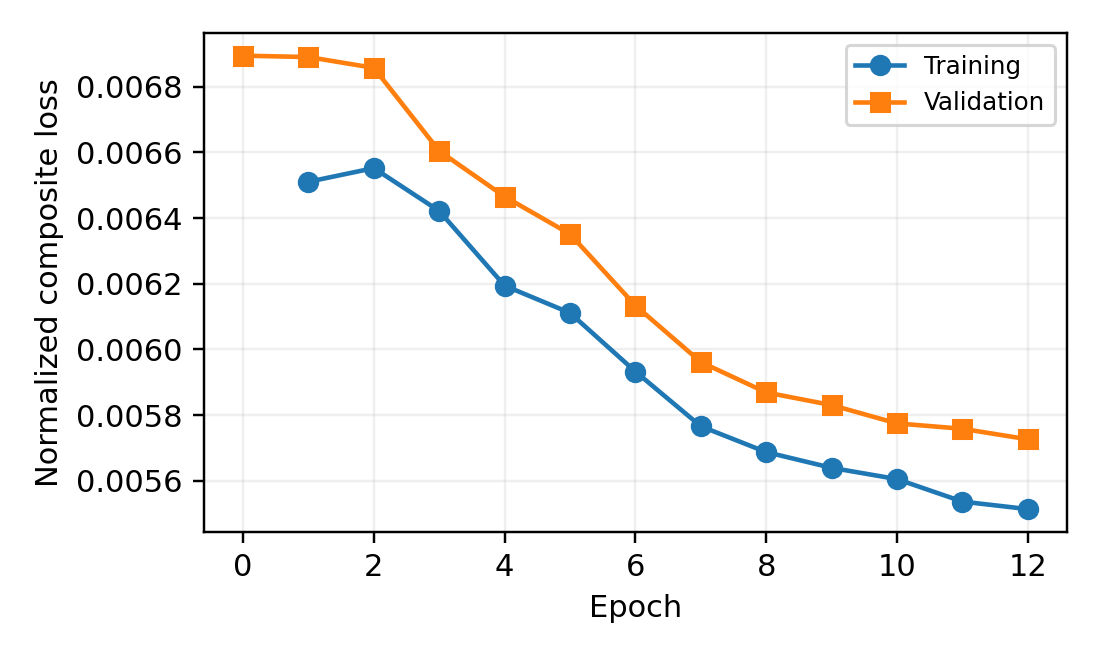
\includegraphics[width=\columnwidth]{figures/learning.png}
\caption{Normalized training and validation composite loss.}
\label{fig:learning}
\end{figure}

The preceding epoch-8 model had failed frozen transfer on one central NMC crop: raw output was 115.41\% worse than SIRT20, and the hybrid 19.19\% worse than SIRT23. This was a different checkpoint and a consumed crop. The new NMC training pilot does not erase that transfer failure.

\subsection{Noise sensitivity}

\begin{table}[!t]
\caption{Frozen noise sensitivity}
\label{tab:noise}
\centering\small
\begin{tabular}{lrrr}
\toprule
Noise & Runs & Raw gain & Hybrid gain \\
\midrule
0\% & 6 & 34.17\% & 35.03\% \\
1\% & 18 & 16.26\% & 15.53\% \\
3\% & 18 & 9.67\% & 9.08\% \\
5\% & 18 & 8.75\% & 8.19\% \\
\bottomrule
\end{tabular}

\end{table}

Hybrid gains decline from 35.03\% at zero noise to 8.19\% at 5\% noise, while remaining positive in the aggregate. Region-mean hybrid wins are 6/6 at each level. The raw method has lower aggregate voxel RMSE than the hybrid at nonzero noise, so three data-fitting steps do not uniformly improve reference fidelity. Gaussian sensitivity is not a calibrated photon-noise or scanner-dose evaluation.

\begin{figure}[!t]\centering
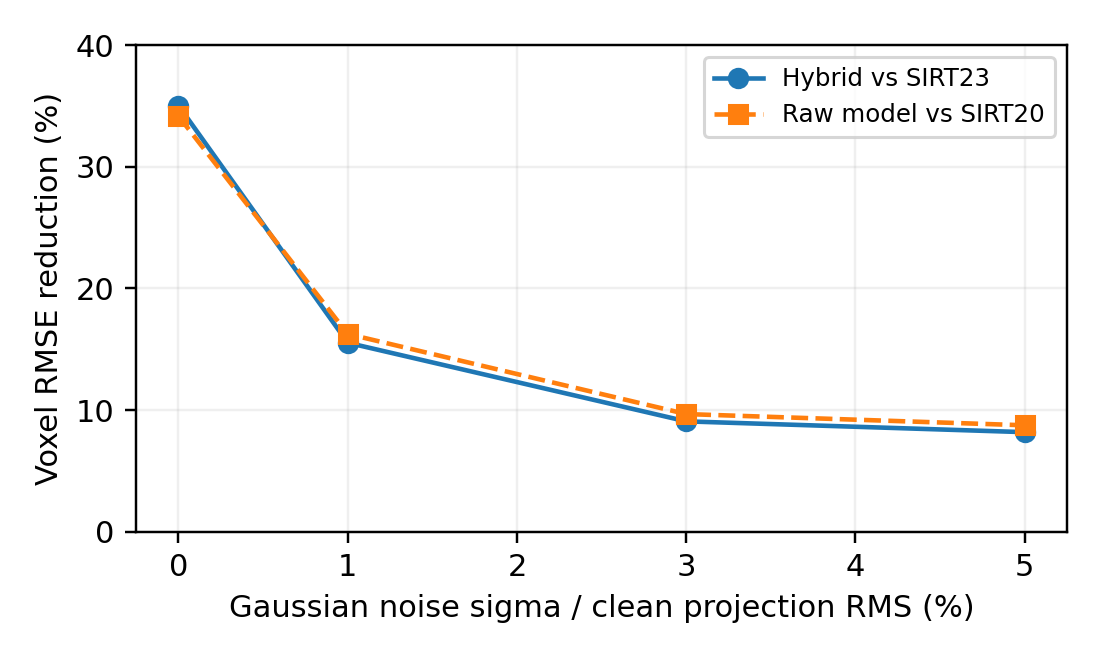
\includegraphics[width=\columnwidth]{figures/noise.png}
\caption{Simulated voxel-error reduction versus Gaussian noise.}
\label{fig:noise}
\end{figure}

\subsection{Measured Waygate model replay}

\begin{table}[!t]
\caption{Measured fit projection RMSE}
\label{tab:measured}
\centering\small
\begin{tabular}{lr}
\toprule
Method & Fit RMSE \\
\midrule
sirt20 & 0.057630 \\
model\_raw & 0.062314 \\
sirt23 & 0.055724 \\
model\_sirt3 & 0.058574 \\
\bottomrule
\end{tabular}

\end{table}

The NMC hybrid has fit projection RMSE 0.058574 versus 0.055724 for SIRT23, a 5.11\% increase. The raw NMC model is also worse than SIRT20 in this replay. This is an observed failure to improve measured-data fit, not proof that its voxel accuracy is lower, because no independent voxel truth is available. The recorded pipeline processing time is 3.112 s, including 1.694 s cold loading/warmup and 0.292 s model inference. Acquisition and archived projection preparation are excluded.

\subsection{View count and voxel resolution}

The controlled FDK comparisons keep preprocessing and approximate geometry fixed. More views reduce streaks, and changing from 128 cubed to 256 cubed makes layers better resolved. The 1200-view 256-cubed result visibly retains layered structure. These observations support angular undersampling and voxel resolution as important causes of lost detail, without confirming calibration.

\begin{table}[!t]
\caption{256-cubed FDK view-count diagnostic}
\label{tab:views}
\centering\small
\begin{tabular}{lrr}
\toprule
Views & Time (s) & Axial RMSE \\
\midrule
75 & 0.211 & 0.023706 \\
150 & 0.231 & 0.012385 \\
300 & 0.271 & 0.003945 \\
600 & 0.358 & 0.001060 \\
1200 & 0.534 & 0.000000 \\
\bottomrule
\end{tabular}
\par\smallskip\footnotesize Axial RMSE is against the same-scan 1200-view FDK, not independent truth.
\end{table}

\begin{figure}[!t]\centering
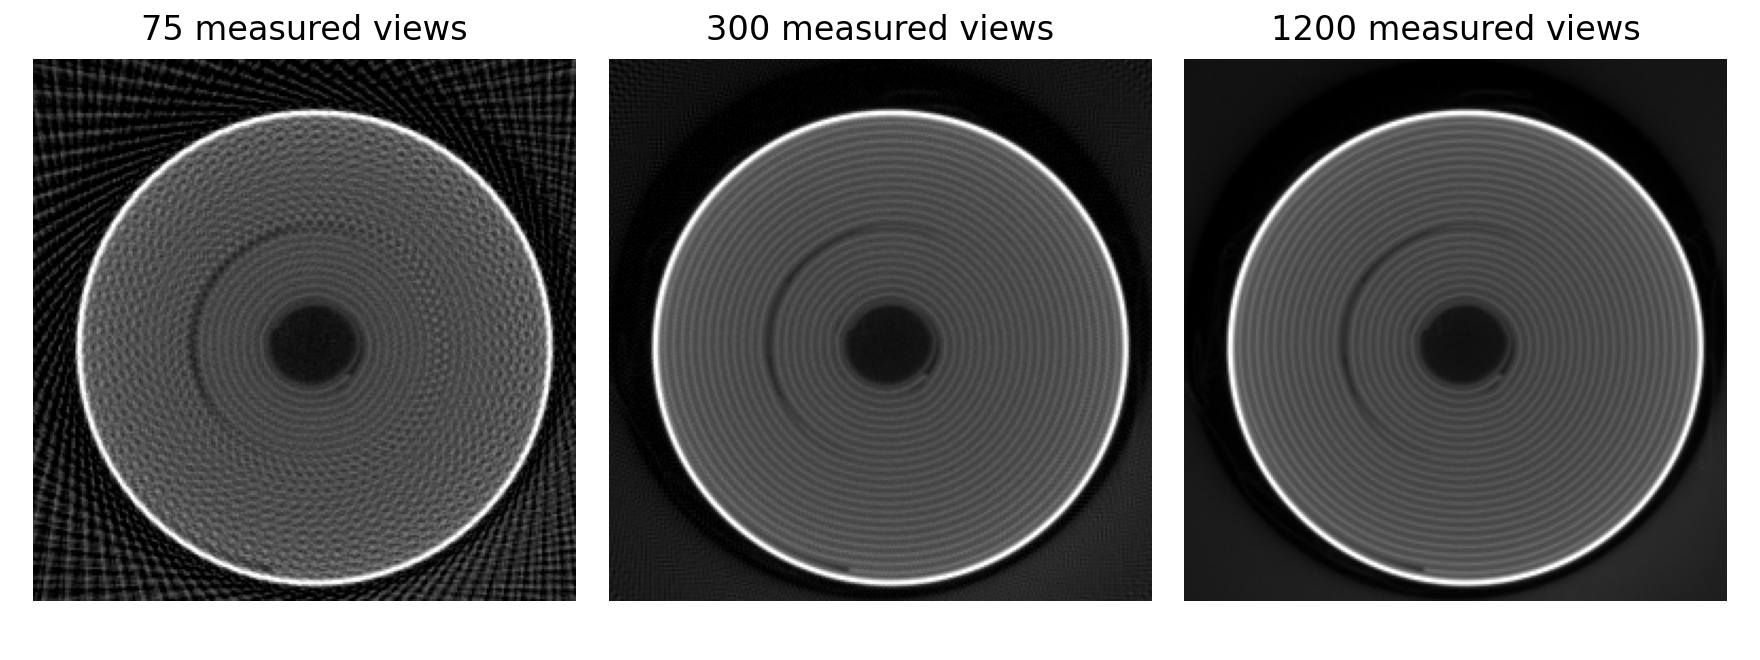
\includegraphics[width=\columnwidth]{figures/views.png}
\caption{Saved middle axial FDK slices; common brightness scale. 75 views show strong streaks; 300 and 1200 views reveal layers.}
\label{fig:views}
\end{figure}

The 75- and 1200-view 256-cubed middle slices reproduce the preceding diagnostic exactly, and the 1200 source-hash manifest matches. The 300-view slice is a useful preview candidate; 600 views is cleaner and closer to the full-view reference. These are provisional presentation choices, not defect-preservation thresholds. Single-run FDK timings exclude capture, preprocessing, display, and packaging; warmup and scheduling effects prevent treating the measured timings as a definitive speed scaling curve.

\section{System And Interactive Interfaces}

The system separates reference/simulation inputs, measured projection preparation, GPU reconstruction, optional frozen correction, reporting, and visualization. The local inference app offers dependency checks, background progress/cancellation, simulation noise controls, tiled prediction, saved volumes, and result ZIP exports. It reports its model identity and processing scope. A separate archive replay application accepts only explicitly acknowledged provisional assumptions.

The latest offline review page embeds the five view-count results and three middle directions. It supports common brightness controls, a comparison overlay, provisional 300-view Preview and 600-view Review choices, image export, a numerical results table, a JSON summary, and a plain-language explanation. It does not execute reconstruction or accept live scanner data. Downloaded comparison images remain views of saved results.

Reproducibility records include fixed region coordinates, source/checkpoint/protocol SHA-256 hashes, selected image indices, acquisition-log angles and timestamps, library versions, finite-array checks, matched extra iterations, and explicit evaluation scope \cite{ref10}. The project environment reports PyTorch 2.11.0+cu128 and ASTRA 2.5.0. An archived geometry report identifies an NVIDIA RTX 2000 Ada Generation GPU; timings are device- and run-dependent.

\section{Challenges And Validity Limits}

The principal scientific challenges are scan-specific correlation, learned domain shift, imperfect simulator realism, uncertain measured-data correction, and the difference between projection consistency and structural accuracy. Non-overlapping patches are not independent specimens, and fitting projections at reconstruction angles is not held-out validation. All-view development diagnostics now use views that had been reserved in an earlier study; those views cannot be relabeled as fresh evaluation data.

The principal engineering challenges are duplicate archive entries, large TIFF stacks, mismatched calibration-image shapes, incorrect unquoted Windows paths, absent downloaded ZIPs, GPU dependency compatibility, and NumPy scalar serialization. A completed noise run failed when json.dumps encountered an int64 count; converting the count with int(region\_wins) fixed report serialization. This was a packaging defect, not a model error.

Negative FDK values and slightly negative transformed measurements are retained where the algorithm permits them. They are not silently clipped for cosmetic presentation. SIRT non-negativity is a method setting, and display windowing is applied consistently rather than changing numerical data. The vendor image is independently scaled only when used as a contextual illustration.

The experiments have no labeled defects, specimen-level independent validation, calibrated attenuation scale, dynamic volume sequence, or scanner connection. Statistical significance and production reliability are not established. An earlier separate Waygate checkpoint was reported to reduce reserved-view RMSE by 2.53\%; its historical result is not merged with this NMC replay or treated as reproduced by the present diagnostics.

\section{Practical Use And Future Work}

The completed prototype is useful for explaining sparse-view CT, comparing saved reconstructions, testing a learned correction under controlled assumptions, and timing GPU processing. It may serve as a starting point for battery inspection research, but current evidence does not support automatic acceptance/rejection of cells, battery health prediction, safety decisions, or measured acquisition acceleration.

A scanner-connected extension should first establish detector crop/binning, gain and offset handling, geometric scale, center and orientation through documented calibration. Next, it should connect an authorized acquisition source, validate complete and stable file arrival, preserve image-angle synchronization, and monitor lag. Acquisition, transfer, preprocessing, inference, display, and packaging should be timed separately, with cold and warm repeated measurements.

Independent scans should evaluate whether selected view counts preserve the structures required by a defined inspection task. New evaluation data must be separated before tuning. Physics controls should be retained, and any retrained measured-domain model compared using reserved projections and structural reference checks. A 4D extension additionally requires temporal acquisition, motion assumptions, and a dedicated dynamic evaluation.

\section{Conclusion}

A reproducible GPU battery CT prototype was completed with a residual NMC correction model, simulated noise evaluation, measured archive replay, and interactive review. The simulation pilot achieves 37.64\% lower mean voxel RMSE than SIRT23 within one scan and 35.38\% on the separate 2000bar stack. In contrast, the NMC hybrid increases measured Waygate fit projection RMSE by 5.11\%.

Physics-only FDK diagnostics show a useful tradeoff between view count and visible detail at 256 cubed. A 300-view preview and 600-view review are reasonable demo candidates for this scan. The project establishes fast archived reconstruction and review, while calibrated real-time acquisition, defect validation, and specimen-level generalization remain future work.

\IEEEtriggeratref{6}
\begin{thebibliography}{11}

\bibitem{ref1} L. A. Feldkamp, L. C. Davis, and J. W. Kress, "Practical cone-beam algorithm," Journal of the Optical Society of America A, vol. 1, no. 6, pp. 612-619, 1984. doi: 10.1364/JOSAA.1.000612. [Online]. Available: \url{https://doi.org/10.1364/JOSAA.1.000612}.

\bibitem{ref2} W. van Aarle et al., "Fast and flexible X-ray tomography using the ASTRA toolbox," Optics Express, vol. 24, no. 22, pp. 25129-25147, 2016. doi: 10.1364/OE.24.025129. [Online]. Available: \url{https://doi.org/10.1364/OE.24.025129}.

\bibitem{ref3} ASTRA Toolbox, "FDK\_CUDA" and "SIRT3D\_CUDA," version 2.5.0 documentation. Accessed Oct. 4, 2026. [Online]. Available: \url{https://astra-toolbox.com/docs/algs/SIRT3D_CUDA.html}.

\bibitem{ref4} O. Cicek, A. Abdulkadir, S. S. Lienkamp, T. Brox, and O. Ronneberger, "3D U-Net: Learning dense volumetric segmentation from sparse annotation," arXiv:1606.06650, 2016. [Online]. Available: \url{https://arxiv.org/abs/1606.06650}.

\bibitem{ref5} K. He, X. Zhang, S. Ren, and J. Sun, "Deep residual learning for image recognition," arXiv:1512.03385, 2015. [Online]. Available: \url{https://arxiv.org/abs/1512.03385}.

\bibitem{ref6} K. H. Jin, M. T. McCann, E. Froustey, and M. Unser, "Deep convolutional neural network for inverse problems in imaging," IEEE Transactions on Image Processing, vol. 26, no. 9, pp. 4509-4522, 2017. doi: 10.1109/TIP.2017.2713099. [Online]. Available: \url{https://doi.org/10.1109/TIP.2017.2713099}.

\bibitem{ref7} A. Paszke et al., "PyTorch: An imperative style, high-performance deep learning library," Advances in Neural Information Processing Systems, vol. 32, 2019. [Online]. Available: \url{https://papers.nips.cc/paper_files/paper/2019/hash/bdbca288fee7f92f2bfa9f7012727740-Abstract.html}.

\bibitem{ref8} K. Mader, "Battery 3D Images," Kaggle dataset. Accessed Oct. 4, 2026. Local experiments use the NMC\_90wt\_0bar and NMC\_90wt\_2000bar grayscale stacks. [Online]. Available: \url{https://www.kaggle.com/datasets/kmader/battery-3d-images}.

\bibitem{ref9} E. Zwanenburg and J. Warnett, "XCT datasets of battery for reconstruction," Zenodo, version v1, 2025. doi: 10.5281/zenodo.14993742. [Online]. Available: \url{https://zenodo.org/records/14993742}.

\bibitem{ref10} A. P. K. Goud, "Sparse4D battery extension experiment records," unpublished project archive, Oct. 4, 2026. Includes protocols, checkpoint hashes, training and noise reports, archived replay results, and view-count diagnostics.

\bibitem{ref11} IEEE Author Center, "Authoring tools and templates," conference author resources. Accessed Oct. 4, 2026. [Online]. Available: \url{https://conferences.ieeeauthorcenter.ieee.org/write-your-paper/authoring-tools-and-templates/}.

\end{thebibliography}

\end{document}